\documentclass{article}

\usepackage[brazil]{babel}

\usepackage{amsmath, amssymb}
\usepackage{graphicx}
\usepackage[colorlinks=true, allcolors=blue]{hyperref}

\usepackage{listings}
\lstset{
basicstyle=\small\ttfamily,
columns=flexible,
breaklines=true
}

\usepackage[section]{placeins}

\usepackage{tcolorbox}

\title{Relatório 03}
\author{Vinícius de Oliveira Peixoto Rodrigues (245294)}
\date{Março de 2023}

\begin{document}
\maketitle

\section{Introdução}

A tecnologia Wi-Fi é uma família de protocolos de rede sem fio, baseadas
na série de padrões IEEE 802.11, que definem as especificações para implementação
de tecnologias de rede wireless. As redes wireless são amplamente utilizadas para
construir redes de pequeno porte em aplicações domésticas ou de negócios.

A ferramenta \texttt{mininet} fornece um conjunto de ferramentas (disponibilizadas
como uma interface de linha de comando ou como uma interface em Python) que permite
a construção de arquiteturas de rede simuladas de forma rápida e fácil. Um fork dessa
ferramenta, chamado \texttt{mininet-wifi}, extende as funcionalidades da ferramenta
original, implementando suporte para simulação de redes Wi-Fi. Este experimento
busca explorar as funcionalidades da ferramenta \texttt{mininet-wifi}.

\section{Objetivos}

Este experimento básico tem como objetivo os seguintes pontos:

\begin{itemize}
    \item Explorar as funcionalidades da ferramenta \texttt{mininet-wifi}
    \item Compreender os princípios básicos de funcionamento de arquiteturas
          de rede wireless
    \item Fazer uso do simulador para investigar a relação entre parâmetros
          físicos e a performance de redes sem fio
\end{itemize}

\section{Metodologia}

O experimento dividiu-se em sete etapas:

\subsection{Primeiros passos}

Foi realizada a criação de uma topologia wireless básica, com um AP e duas estações
(\texttt{sta1} e \texttt{sta2}).
Em seguida, foram realizados testes básicos de conexão e desconexão entre as estações
e o access point; finalmente, foram realizadas medições de largura de banda entre as
duas estações.

\subsection{Exploração dos parâmetros do simulador}
Foi explorado o ajuste de parâmetros das estações no simulador, em particular o de
posição das estações. Além disso, foi realizada uma análise dos diversos parâmetros
de configuração disponíveis no simulador.


\subsection{Visualização da topologia wireless}

Nesta etapa, foram feitos testes com diferentes esquemas
de plotagem de topologias wireless disponíveis no mininet-wifi.


\subsection{Análise de frames MAC 802.11}

Já aqui, foi investigado por meio da ferramenta Wireshark
o formato de frames padrão 802.11, e como ele difere dos
frames 802.3.

\subsection{Estudo de modelos de propagação}

Nesta etapa, foi investigada a influência de diferentes
modelos teóricos de propagação de sinal na comunicação
entre estações e APs Wi-Fi.

\subsection{Análise da influência do RSSI na bandwidth}

Em seguida, foi analisado, utilizando-se um dos modelos
investigados na etapa interior, a influência do RSSI no
throughput de comunicação entre duas estações na rede Wi-Fi,
à medida que uma delas se distancia do AP.

\subsection{Investigação do \textit{Roaming} Wi-Fi}

Finalmente, foi estudado um caso de simulação no \texttt{mininet-wifi}
que demonstra o comportamento do \textit{roaming} quando uma
estação transita entre as regiões de cobertura de dois APs
diferentes (mas com mesmo SSID).


\section{Resultados e Discussão}

\subsection*{Parte 1}

\begin{tcolorbox}
    Qual é o atraso observado entre \texttt{sta1} e \texttt{sta2}?
    Houve perda de pacotes no canal? Justifique suas respostas de forma objetiva.
\end{tcolorbox}

\begin{figure}[!htb]
\centering
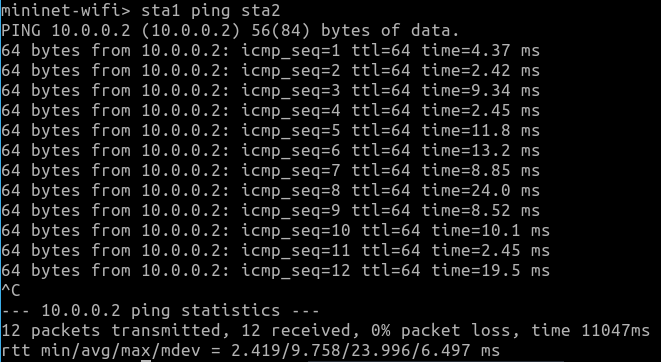
\includegraphics[width=\columnwidth]{images/p1_ping.png}
\caption{\texttt{ping} entre \texttt{sta1} e \texttt{sta2}.}
\end{figure}

O atraso médio observado na saída do comando \texttt{ping} é de 9.8 segundos.
Além disso, não foram observadas perdas de pacote.

\begin{tcolorbox}
    Use a ferramenta iperf para avaliar a banda disponível (Mbps)
    entre sta1 e sta2.
\end{tcolorbox}

\begin{figure}[!htb]
\centering
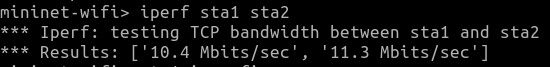
\includegraphics[width=\columnwidth]{images/p1_iperf.png}
\caption{Teste de largura de banda entre \texttt{sta1} e \texttt{sta2}.}
\end{figure}

\begin{figure}[!htb]
\centering
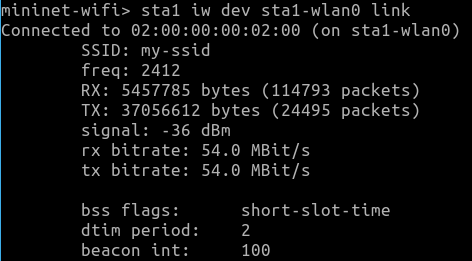
\includegraphics[width=\columnwidth]{images/p1_iwconfig.png}
\caption{Status do link \texttt{wlan} da estação \texttt{sta1}, demonstrando velocidade negociada maior do que a medida pelo \texttt{iperf}.}
\end{figure}

A largura de banda média entre as duas estações é de aproximadamente 11 Mbits/sec.
É interessante observar que a largura de banda na prática é significativamente menor que o
bitrate máximo negociado para os links \texttt{wlan} de cada estação.


\FloatBarrier

\subsection{Análise de quadros}
Análise de quadros 802.11 gerados pelo simulador no Wireshark

\subsection*{Parte 2}

\begin{tcolorbox}
    Identifique a posição dos nós \texttt{sta1} e \texttt{sta2}.
\end{tcolorbox}

\begin{figure}[!htb]
\centering
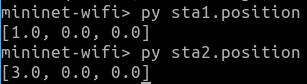
\includegraphics[width=\columnwidth]{images/p2_position.png}
\caption{Posição das estações \texttt{sta1} e \texttt{sta2}.}
\end{figure}

\FloatBarrier

\begin{tcolorbox}
    Investigue a lista de parâmetros de \texttt{sta1} (\texttt{py sta1.params}).
    Explique resumidamente qual informação do nó \texttt{sta1} cada item da lista representa.
\end{tcolorbox}

\begin{figure}[!htb]
\centering
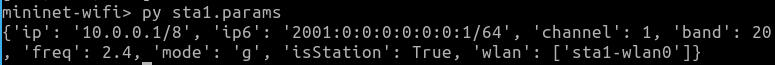
\includegraphics[width=\columnwidth]{images/p2_params.png}
\caption{Parâmetros de \texttt{sta1}.}
\end{figure}

Os parâmetros encontrados são:

\begin{itemize}
    \item \texttt{ip}/\texttt{ip6}: o endereço IPv4/Ipv6 atribuído à interface \texttt{wlan}
          da estação
    \item \texttt{channel}: o canal (isto é, faixa de frequências de operação) de
          acordo com a especificação 802.11g
    \item \texttt{band}: a banda (2.4 GHz) de comunicação wireless
    \item \texttt{freq}: a frequência da comunicação wireless
    \item \texttt{mode}: qual versão específica do protocolo 802.11 (neste caso,
          802.11g) na qual o canal está operando
    \item \texttt{isStation}: variável para identificação de estações Wi-Fi
    \item \texttt{wlan}: indica qual interface de rede (\texttt{sta1-wlan0}) está
          sendo usada para a conexão Wi-Fi


\end{itemize}

\subsection{Parte 3}

\begin{tcolorbox}
    Plote um gráfico em duas e outro em três dimensões.
\end{tcolorbox}

\begin{figure}[!htb]
\centering
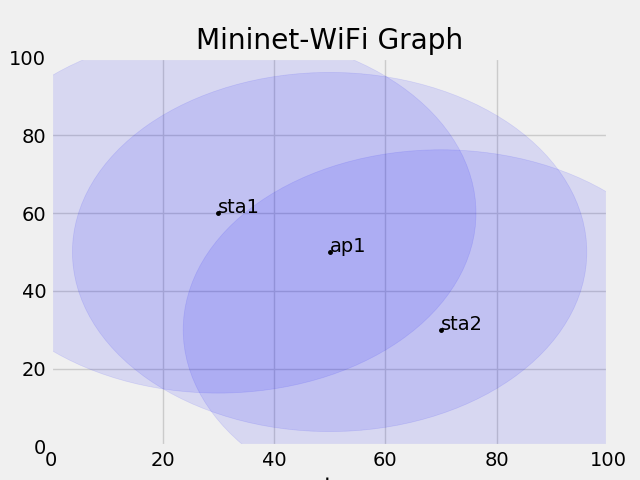
\includegraphics[width=0.6\columnwidth]{images/p3_2d.png}
\caption{Gráfico 2D gerado.}
\end{figure}

\begin{figure}[!htb]
\centering
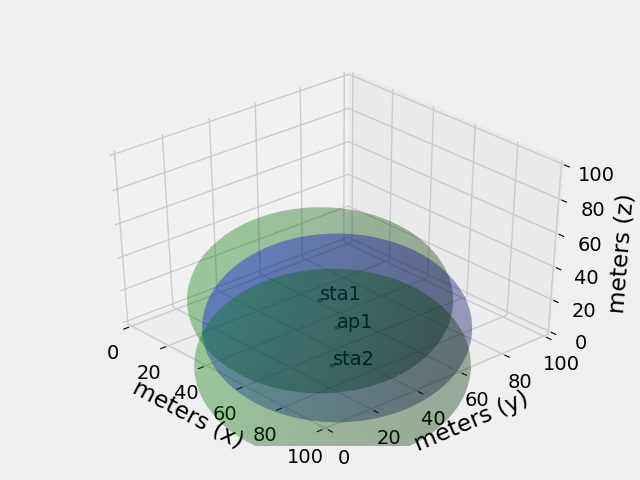
\includegraphics[width=0.6\columnwidth]{images/p3_3d.png}
\caption{Gráfico 3D gerado.}
\end{figure}

\FloatBarrier

\subsection{Parte 4}

\begin{tcolorbox}
    Explique as principais diferenças e funções em relação ao número de endereços MAC contidos nos quadros do tipo 802.11 e 802.3.
\end{tcolorbox}

\begin{figure}[!htb]
\centering
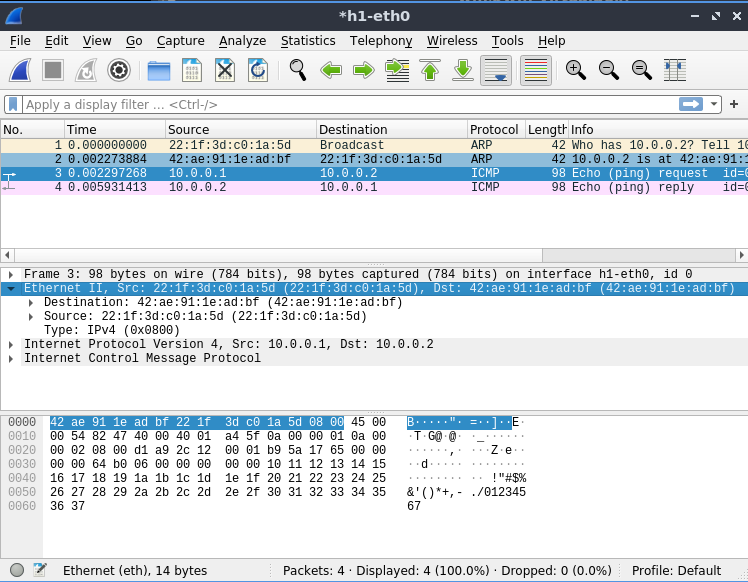
\includegraphics[width=0.8\columnwidth]{images/p4_wired.png}
\caption{Frame MAC numa conexão \textit{wired}.}
\label{fig:p4_wired}
\end{figure}

\begin{figure}[!htb]
\centering
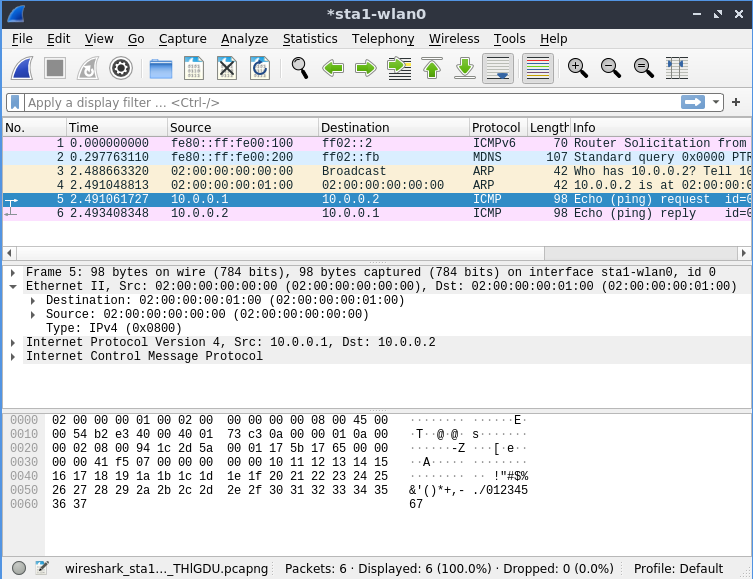
\includegraphics[width=0.8\columnwidth]{images/p4_wireless.png}
\caption{Frame MAC numa conexão \textit{wireless}.}
\label{fig:p4_wireless}
\end{figure}


Um frame 802.11 contém, além dos endereços MAC
\texttt{source} e \texttt{destination} encontrados
no 802.3, um terceiro endereço MAC pertencente ao
\textit{access point}.

As Figuras \ref{fig:p4_wired} e \ref{fig:p4_wireless}
mostram, contudo, que na captura de pacotes do Wireshark
os frames MAC com fio e sem fio são idênticos; isso
acontece porque a interface \textit{wireless} do
\texttt{mininet-wifi} está rodando em modo \textit{managed},
o que significa que o driver da interface no kernel
"reorganiza" os
frames MAC dos pacotes que entram e saem, retirando os
campos específicos do 802.11 e substituindo pelos
equivalentes no 802.3; não foi possível rodar a interface
simultaneamente em modo monitor e managed para ilustrar
as diferenças de frames no 802.11 e 802.3.

\FloatBarrier

\subsection{Parte 5}

\begin{tcolorbox}
    Um dos nós parece estar incomunicável. Qual é ele e por qual motivo o nó está incomunicável? Ele encontra-se associado ao AP1?
\end{tcolorbox}

\begin{figure}[!htb]
\centering
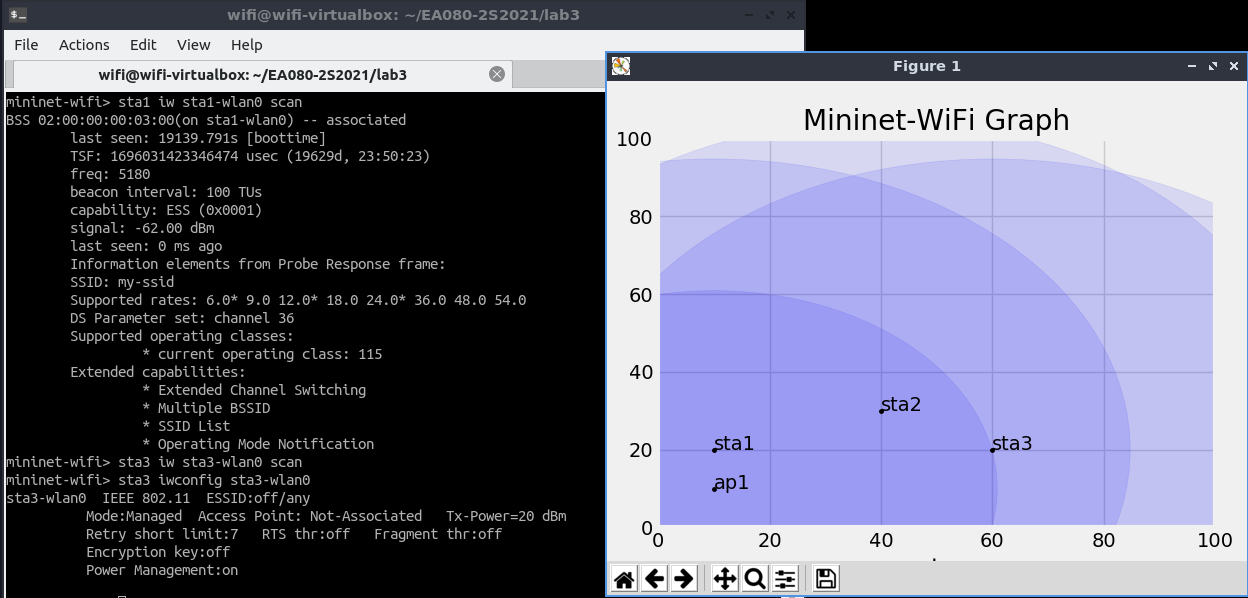
\includegraphics[width=0.8\columnwidth]{images/p5_scan.png}
\caption{Diagnóstico da estação \texttt{sta3}, que se encontra incomunicável.}
\label{fig:p5_scan}
\end{figure}

Na Figura \ref{fig:p5_scan}, é possível ver que a estação
\texttt{sta3} se encontra inalcançável, visto que não está
associada ao AP \texttt{ap1}. Isso acontece, como ilustrado
no gráfico, porque \texttt{sta3} está fora do alcance de
\texttt{ap1} (razão pela qual o AP aparece no scan de
\texttt{sta1}, mas não de \texttt{sta3}).

\begin{tcolorbox}
    O script já vem pré-configurado com um modelo de propagação. Identifique-o.
\end{tcolorbox}

\begin{figure}[!htb]
\centering
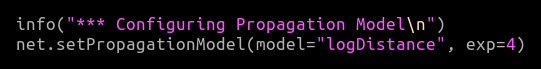
\includegraphics[width=0.8\columnwidth]{images/p5_logdistance.png}
\caption{Modelo de propagação selecionado no código.}
\label{fig:p5_logdistance}
\end{figure}

A Figura \ref{fig:p5_logdistance} mostra o snippet
de código relevante, onde é configurado o modelo
\href{https://en.wikipedia.org/wiki/Log-distance_path_loss_model}{Log-distance path loss}, onde a potência do sinal cai exponencialmente:

\begin{equation*}
    \frac{P_{\text{Rx}}}{P_{\text{Tx}}} \sim \frac{1}{d^\gamma}
\end{equation*}

\begin{tcolorbox}
    Identifique e descreva o nível de sinal percebido por sta1. Depois substitua o modelo de propagação do script por um outro suportado pelo Mininet-WiFi e então configure esse modelo no script.
\end{tcolorbox}

\begin{figure}[!htb]
\centering
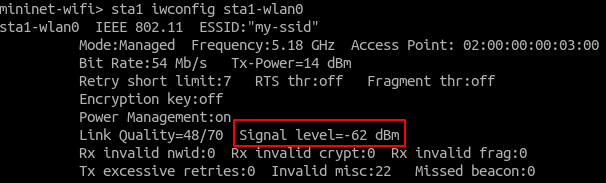
\includegraphics[width=0.8\columnwidth]{images/p5_signal_level_before.png}
\caption{Nível de sinal para o modelo log-distance.}
\label{fig:p5_signal_level_before}
\end{figure}

O outro modelo de propagação escolhido foi o \href{https://en.wikipedia.org/wiki/Friis_transmission_equation}{Friis path loss},
no qual a potência do sinal cai com o quadrado da distância:

\begin{equation*}
    \frac{P_{\text{Rx}}}{P_{\text{Tx}}} \sim \frac{1}{d^2}
\end{equation*}

\begin{figure}[!htb]
\centering
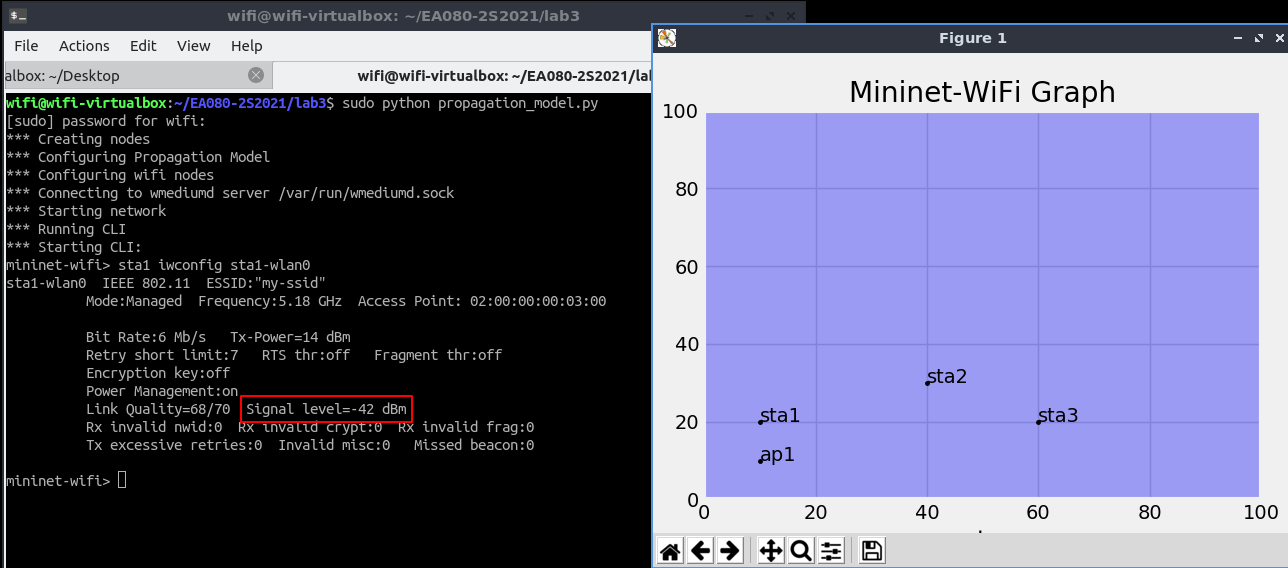
\includegraphics[width=0.8\columnwidth]{images/p5_signal_level_after.png}
\caption{Nível de sinal para o modelo Friis.}
\label{fig:p5_signal_level_after}
\end{figure}

\begin{tcolorbox}
    Há diferenças entre o nível de sinal antes e após a mudança do modelo de propagação? Justifique o resultado obtido.
\end{tcolorbox}

Sim: percebe-se que o nível de sinal aumentou com o uso do modelo
de propagação Friis ($-62 \text{dB} \rightarrow -42 \text{dB}$).

\subsection{Parte 6}

\begin{tcolorbox}
Com o script \texttt{propagation\_model.py} e utilizando Iperf, monte um gráfico ou tabela que relacione a largura de banda entre dois nós (sta) com a distância x entre eles, assim como exemplificado na figura. Monte também um gráfico ou tabela que relacione o nível de sinal à distância.
\end{tcolorbox}

Para essa etapa, foi utilizado o modelo Fiis de propagação.
O script \texttt{propagation\_model.py} (enviado em anexo
juntamente ao relatório)
foi modificado para
aumentar gradualmente a distância entre as estações e
coletar dados de RSS e throughput.

\begin{figure}[!htb]
\centering
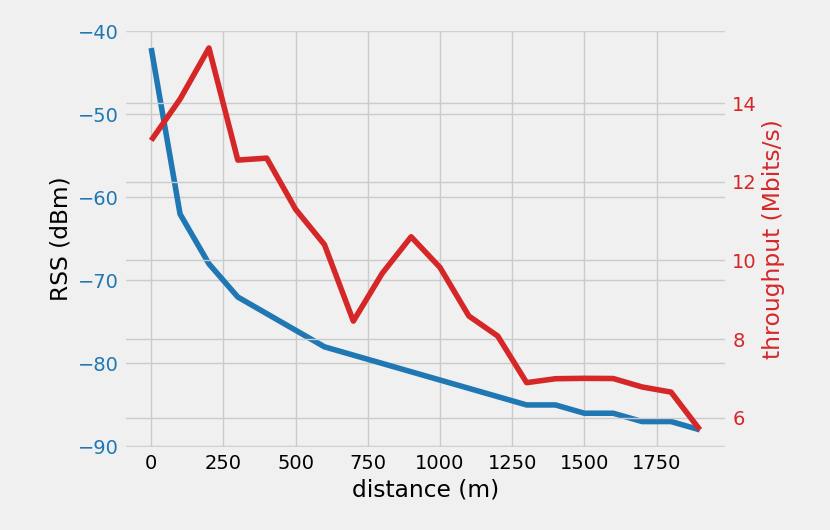
\includegraphics[width=\columnwidth]{images/p6_plot.png}
\caption{Influência do RSS no throughput entre as estações.}
\label{fig:p6_plot}
\end{figure}


Na Figura \ref{fig:p6_plot}, apesar das variações aleatórias
introduzidas pela simulação do \texttt{mininet-wifi},
é possível ver que a
diminuição do RSS devido ao distanciamento entre
\texttt{sta1} e \texttt{sta2} faz com que o throughput
entre da comunicação entre as estações seja deteriorado.

\subsection{Parte 7}

\begin{tcolorbox}
    A comunicação entre sta1 e sta2 se manteve ininterrupta? Por quê? O que aconteceu com sta1?
\end{tcolorbox}

Não; a Figura \ref{fig:p7_disconnection} mostra o momento
em que houve uma desconexão quando \texttt{sta1}
saiu da área de alcance do \texttt{ap1} e entrou na área
de cobertura do \texttt{ap2}, desconectando-se de um para
conectar-se ao outro.

\begin{figure}[!htb]
\centering
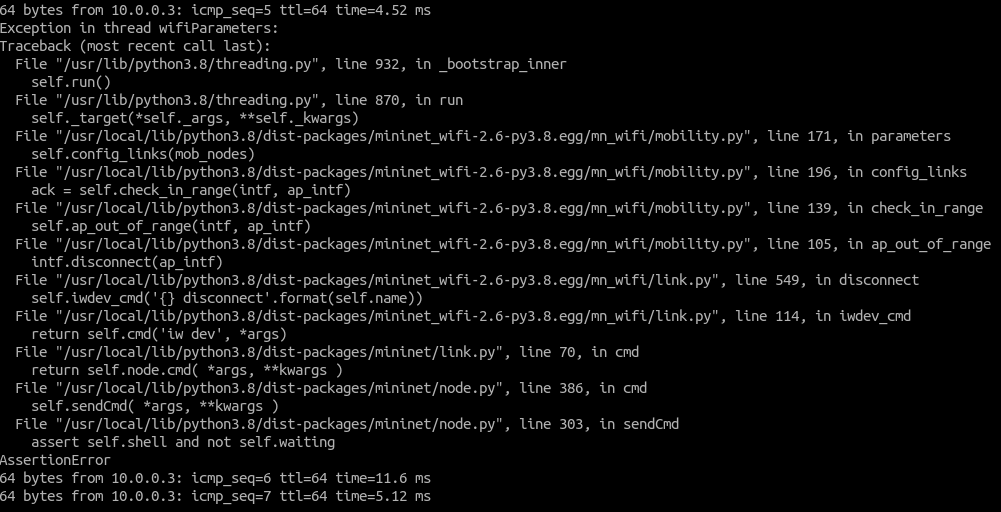
\includegraphics[width=\columnwidth]{images/p7_disconnection.png}
\caption{Desconexão durante o processo de movimentação de \texttt{sta1} entre a cobertura dos APs.}
\label{fig:p7_disconnection}
\end{figure}

\begin{tcolorbox}
    Qual o nome do processo que a mobilidade ocasionou em sta1 ? Comente como ele funciona.
\end{tcolorbox}

O nome do processo é \textit{roaming}; essencialmente,
as estações costumam definir um \textit{roaming threshold}
para o RSSI com o AP atual; quando o RSSI se torna ruim
o suficiente de modo a passar desse limite, a estação começa
a fazer \textit{scans} de modo a procurar outros APs com
o mesmo SSID do atual. A estação escolhe então o AP
alternativo com maior RSSI, e se conecta a ele.

\end{document}
